\chapter{Μεθοδολογία}
\label{ch:methodology}

\section{Στοιχειώδεις Γεωμετρικές Πράξεις}
\subsection{Ευκλείδεια Απόσταση δύο Τριγώνων}
\label{subsec:tria_distance}
% Έστω τα τρίγωνα $P$ και $Q$ στον $\mathbb{R}^3$.
% Η Ευκλείδεια απόσταση $d(P,Q)$ μεταξύ των τριγώνων $P$ και $Q$
% ορίζεται ως:
% \[ d(P,Q) = \min_{p \in P, q \in Q} |p - q| \]
% όπου με $|p-q|$ συμβολίζεται η Ευκλείδεια απόσταση των σημείων 
% $p$ και $q$.

% Έστω p,q

\subsubsection{Ευκλείδεια Απόσταση δύο Ευθυγράμμων Τμημάτων}
\subsubsection{Ευκλείδεια Απόσταση Σημείου και Τριγώνου}

\subsection{Γεωμετρικές Πράξεις για \tl{AABB}}
Ένα οριοθετικό πλαίσιο ευθυγραμμισμένο με τους άξονες (\tl{AABB})
είναι, απλώς, ένα ορθογώνιο παραλληλεπίπεδο του οποίου οι 
έδρες είναι κάθετες σε ένα από τα διανύσματα βάσης.

Ένα \tl{AABB} αναπαριστάται στη μνήμη από τα άκρα της κύριας 
διαγωνίου του.
Δηλαδή το σημείο $S$ με τις μικρότερες $x$, $y$, $z$ συντεταγμένες
και το σημείο $T$ με τις μεγαλύτερες $x$, $y$, $z$ συντεταγμένες.

\begin{figure}[h]
    \centering
    
    \newcommand{\Depth}{2}
    \newcommand{\Height}{2}
    \newcommand{\Width}{3}
    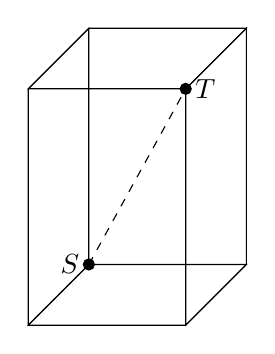
\begin{tikzpicture}
        \coordinate (O) at (0,0,0);
        \coordinate (A) at (0,\Width,0);
        \coordinate (B) at (0,\Width,\Height);
        \coordinate (C) at (0,0,\Height);
        \coordinate (D) at (\Depth,0,0);
        \coordinate (E) at (\Depth,\Width,0);
        \coordinate (F) at (\Depth,\Width,\Height);
        \coordinate (G) at (\Depth,0,\Height);

        \draw[] (O) -- (C) -- (G) -- (D) -- cycle;% Bottom Face
        \draw[] (O) -- (A) -- (E) -- (D) -- cycle;% Back Face
        \draw[] (O) -- (A) -- (B) -- (C) -- cycle;% Left Face
        \draw[] (D) -- (E) -- (F) -- (G) -- cycle;% Right Face
        \draw[] (C) -- (B) -- (F) -- (G) -- cycle;% Front Face
        \draw[] (A) -- (B) -- (F) -- (E) -- cycle;% Top Face

        \draw[fill=black] (O) circle (2pt) node[left]{$S$};
        \draw[fill=black] (F) circle (2pt) node[right]{$T$};
        \draw[dashed] (O) -- (F);
    \end{tikzpicture}
    \caption[Αναπαράσταση ενός \tl{AABB}]{Αναπαράσταση ενός \tl{AABB}}
\end{figure}

\subsubsection{Υπολογισμός Απόστασης \tl{AABB-AABB}}
Έστω τα ευθυγραμμισμένα με τους άξονες πλαίσια
$P$ και $Q$ στον $\mathbb{R}^3$.
Η Ευκλείδεια απόσταση $d(P,Q)$ μεταξύ των πλαισίων $P$ και $Q$
ορίζεται ως:
\[ d(P,Q) = \min_{p \in P, q \in Q} \lVert p - q \rVert \]
όπου με $\lVert p - q \rVert$ συμβολίζεται η Ευκλείδεια 
απόσταση των σημείων $p$ και $q$.

Για τον υπολογισμό της απόστασης μεταξύ δύο τέτοιων πλαισίων, 
εκμεταλλευόμαστε το γεγονός ότι οι πλευρές τους είναι ευθυγραμμισμένες
με του άξονες.
Έτσι μπορούμε να υπολογίσουμε την απόσταση χωρίζοντας τη στις συνιστώσες της.
Τελικά, προκύπτει ο αλγόριθμος \ref{alg:aabb_dist}, 
όμοιος με αυτόν που περιγράφεται στο \cite{krishnamurthy2011gpu}.
Στον παραπάνω αλγόριθμο  ο τελεστής "$-$" στις γραμμές 
$1$,$2$ είναι διανυσματική αφαίρεση των συντεταγμένων των σημείων.
Ο τελεστής \tl{\texttt{max(0, $v$)}} είναι επίσης διανυσματικός και
αντικαθιστά όλες τις αρνητικές τιμές ενός διανύσματος $v$
με $0$.
Ο τελεστής $\cdot$ είναι το εσωτερικό γινόμενο διανυσμάτων.

\selectlanguage{english}
\IncMargin{1.5em}
\begin{algorithm}[H]
    \label{alg:aabb_dist}
    \caption[Υπολογισμός Απόστασης δύο \tl{AABB}]{
        \tg{Υπολογισμός της Ευκλείδειας Απόστασης δύο AABB}
    }
    \DontPrintSemicolon
    \KwIn{Two AABBs $P$, $Q$}
    \KwOut{Euclidean Distance of $P$ and $Q$}
    \SetKwFunction{funcname}{AABB\_distance}
    \SetKwFunction{max}{max}
    \Indm\nonl\funcname($P$, $Q$)\\
    \Indp
        $w \gets \max(0, P.S - Q.T)$\;
        $v \gets \max(0, Q.S - P.T)$\;
        \Return{$\sqrt{v \cdot v + w \cdot w}$}

    
\end{algorithm}
\DecMargin{1.5em}
\selectlanguage{greek}

\subsubsection{Κατασκευή \tl{AABB} Από Τρίγωνο}
Με τον αλγόριθμο \ref{alg:aabb_from_triangle} κατασκευάζουμε 
ένα \tl{AABB} που εξ' ολοκλήρου περικλείει ένα τρίγωνο.
Η ρουτίνα \tl{\texttt{vertices($T$)}} επιστρέφει τις 
τρεις κορυφές του τριγώνου $T$.
Οι τελεστές \tl{\texttt{min(), max()}} είναι διανυσματικοί,
δέχονται ως όρισμα μια λίστα από διανύσματα και επιστρέφουν 
ένα διάνυσμα με τις ελάχιστες/μέγιστες συντεταγμένες ανά άξονα.

\selectlanguage{english}
\IncMargin{1.5em}
\begin{algorithm}[H]
    \label{alg:aabb_from_triangle}
    \caption[Κατασκευή \tl{AABB} από Τρίγωνο]{
        \tg{Κατασκευή \tl{AABB} από Τρίγωνο}
    }
    \DontPrintSemicolon
    \KwIn{A Triangle $T$}
    \KwOut{An AABB Enclosing $T$}
    \SetKwFunction{funcname}{AABB}
    \SetKwFunction{min}{min}
    \SetKwFunction{max}{max}
    \SetKwFunction{vertices}{vertices}
    \Indm\nonl\funcname($T$)\\
    \Indp
        $S \gets \min(\vertices(T))$\;
        $T \gets \max(\vertices(T))$\; 
        \Return{ \{$S$, $T$\}}
    
\end{algorithm}
\DecMargin{1.5em}
\selectlanguage{greek}

\subsubsection{Συνένωση Δύο \tl{AABB}}
Ο αλγόριθμος \ref{alg:combine_aabbs} κατασκευάζει ένα \tl{AABB} περικλείει
εξ' ολοκλήρου δύο άλλα \tl{AABB} που δέχεται ως ορίσματα. 
Αυτή η πράξη είναι χρήσιμη γιατί αν έχουμε ήδη βρει τα \tl{AABB} για δύο 
ομάδες αντικειμένων ξεχωριστά, μπορούμε σε σταθερό χρόνο $\bigO(1)$ να 
κατασκευάσουμε το \tl{AABB} που περικλείει όλα τα αντικείμενα. 
Οι τελεστές \tl{\texttt{min(), max()}} είναι ίδιοι με πριν.

\selectlanguage{english}
\IncMargin{1.5em}
\begin{algorithm}[H]
    \label{alg:combine_aabbs}
    \caption[Κατασκευή \tl{AABB} από δύο άλλα \tl{AABB}]{
        \tg{Κατασκευή \tl{AABB} από δύο άλλα \tl{AABB}}
    }
    \DontPrintSemicolon
    \KwIn{Two AABBs $P$, $Q$}
    \KwOut{An AABB Enclosing $P$ and $Q$}
    \SetKwFunction{funcname}{combine\_AABB}
    \Indm\nonl\funcname($P$, $Q$)\\
    \Indp
        
    $S \gets \min(P.S, Q.S)$\;
    $T \gets \max(P.T, Q.T)$\; 
    \Return{ \{$S$, $T$\}}
\end{algorithm}
\DecMargin{1.5em}
\selectlanguage{greek}

\section{Αλγόριθμοι Εξαντλητικής Αναζήτησης}
\label{sec:exhaustive_search}
Έστω δύο αντικείμενα του τρισδιάστατου χώρου που αναπαρίστανται από 
τριγωνικά πλέγματα.
Από τον ορισμό της Ευκλείδειας απόστασης δύο τριγωνικών πλεγμάτων που
δόθηκε στην ενότητα \ref{sec:problem_description} και τη χρήση μιας 
ρουτίνας \tl{\texttt{triangle\_distance(p, q)}}, προκύπτει ο 
τετριμμένος αλγόριθμος \ref{alg:exhaustive_search}. 
Η πολυπλοκότητα του αλγορίθμου είναι $\bigO(N*M)$, όπου 
$N$ και $M$ είναι το πλήθος των τριγώνων των δύο αντικειμένων.

\selectlanguage{english}
\IncMargin{1.5em}
\begin{algorithm}[h]

    \caption[Απόσταση Τριγωνικών Πλεγμάτων με Πλήρη Αναζήτηση]{
        \tg{Απόσταση Τριγωνικών Πλεγμάτων με Πλήρη Αναζήτηση}
    }
    \label{alg:exhaustive_search}
    \DontPrintSemicolon
    \KwIn{Two Triangle Meshes $P$, $Q$}
    \KwOut{Euclidean Distance of $P$ and $Q$}
    \SetKwFunction{dist}{triangle\_distance}
    \SetKwFunction{trias}{triangles}
    \SetKwFunction{min}{min}
    \SetKwFunction{exhaustivesearch}{triangle\_mesh\_distance}
    \Indm\nonl\exhaustivesearch ($P$, $Q$)\\
    \Indp
        $T_P \gets$ \trias($P$) \;
        $T_Q \gets$ \trias($Q$) \; 
        $distance \gets \inf$ \;
        \ForEach{$p \in T_P$}{
            \ForEach{$q \in T_Q$}{
                $distance \gets \min(distance, \dist(p,q))$\;
            }
        }
        \Return{$distance$}
\end{algorithm}
\DecMargin{1.5em}
\selectlanguage{greek}

Σύμφωνα με τη μελέτη που έγινε στην ενότητα \ref{sec:bounding_volumes}
μπορούμε να επιταχύνουμε τον χρόνο εκτέλεσης του αλγορίθμου αν 
χρησιμοποιήσουμε οριοθετικούς όγκους.
Συγκεκριμένα, θα χρησιμοποιήσουμε Οριοθετικά Πλαίσια Ευθυγραμμισμένα 
με τους Άξονες (\tl{AABB}). 
Όπως φαίνεται από τον πίνακα της ενότητας \ref{sec:geom_tests_cost},
ο υπολογισμός της ελάχιστης απόστασης \textit{\tl{AABB - AABB}} είναι πολύ πιο 
"οικονομικός" υπολογιστικά σε σχέση με τον υπολογισμό της απόστασης 
\textit{τρίγωνο - τρίγωνο}.
Μπορούμε να εκμεταλλευτούμε αυτό το γεγονός και σε συνδυασμό με το παρακάτω λήμμα 
να σχεδιάσουμε έναν ταχύτερο αλγόριθμο.

\begin{lemma}
    Έστω δύο σύνολα $S_A$ και $S_B$ που αποτελούνται από χωρικά αντικείμενα. 
    Έστω οι οριοθετικοί όγκοι $BV_A$ και $BV_B$ που εξ' ολοκλήρου περικλείουν 
    τα αντικείμενα των σύνολων  $S_A$ και $S_B$, αντίστοιχα. Τότε:
    
    \[ distance(BV_A, BV_B) \leq distance(a, b) , 
    \forall a \in S_A, \forall b \in S_B \]

    Δηλαδή, η Ευκλείδεια απόσταση οποιουδήποτε ζεύγους αντικειμένων από τα δύο σύνολα 
    θα είναι μεγαλύτερη ή ίση με την Ευκλείδεια απόσταση των οριοθετικών όγκων 
    των συνόλων.
    \label{lemma:box_distance}
\end{lemma}


\begin{proof}
    Συμβολίζουμε με $BV_A$ το σύνολο των σημείων του 
    οριοθετικού όγκου, $BV_A$. 
    Όμοια και για το σύνολο $BV_B$.

    Επίσης, έχουμε
    $S_A = \bigcup\limits_{a \in S_A} a $ και $S_B = \bigcup\limits_{b \in S_B} b$,
    όπου με $a$, $b$ συμβολίζουμε το σύνολο των σημείων των 
    χωρικών αντικειμένων $a$ και $b$.

    Αφού οι οριοθετικοί όγκοι περικλείουν τα σύνολα των 
    αντικειμένων $S_A$ και $S_B$ ισχύει επίσης ότι 
    $S_A \subseteq BV_A $ και 
    $S_B \subseteq BV_B $.

    Έστω ότι υπάρχουν αντικείμενα $a \in S_A$, $b \in S_B$ με απόσταση μικρότερη 
    από αυτή των οριοθετικών όγκων. Τότε, υπάρχουν σημεία $p \in a \subseteq S_A 
    \subseteq BV_A$ και $q \in b \subseteq S_B \subseteq BV_A$ ώστε 
    \[\lVert p - q \rVert < distance(BV_A, BV_B)\]
    Από τον ορισμό της Ευκλείδειας απόστασης δύο οριοθετικών όγκων καταλήγουμε 
    σε άτοπο.
\end{proof}

Προκύπτει, λοιπόν, ο αλγόριθμος \ref{alg:exhaustive_search_aabb}.
Αρχικά, κάθε τρίγωνο περικλείεται από 
ένα \tl{AABB}. Σε κάθε βήμα του αλγορίθμου είναι γνωστή η μικρότερη απόσταση 
που έχει υπολογιστεί μέχρι εκείνη τη στιγμή. Έτσι, για κάθε ζεύγος τριγώνων, 
πρώτα γίνεται ο γρήγορος υπολογισμός απόστασης \tl{AABB-AABB} και μόνο όταν αυτή 
η απόσταση είναι μικρότερη από την τρέχουσα απόσταση γίνεται ο έλεγχος 
τρίγωνο-τρίγωνο.
Η υπολογιστική πολυπλοκότητα παραμένει $\bigO(N*M)$, όπως και πριν.
Σημειώνεται, ότι ο χρόνος εκτέλεσης επηρεάζεται από τη σειρά που θα γίνουν 
οι πράξεις. Δηλαδή αν η μικρότερη απόσταση βρεθεί από πολύ νωρίς, τότε 
θα γίνουν πολύ λίγοι υπολογισμοί τρίγωνο-τρίγωνο, ενώ το αντίθετο θα συμβεί 
αν η μικρότερη απόσταση βρεθεί πιο αργά.

\selectlanguage{english}
\IncMargin{1.5em}
\begin{algorithm}[h]
    \caption[Απόσταση Τριγωνικών Πλεγμάτων με Πλήρη Αναζήτηση και \tl{AABB}]{
        \tg{Απόσταση Τριγωνικών Πλεγμάτων με Πλήρη Αναζήτηση και} AABB
        }
    \label{alg:exhaustive_search_aabb}
    \DontPrintSemicolon
    \KwIn{Two Triangle Meshes $P$, $Q$}
    \KwOut{Euclidean Distance of $P$ and $Q$}
    \SetKwFunction{dist}{triangle\_distance}
    \SetKwFunction{aabbdist}{AABB\_distance}
    \SetKwFunction{trias}{triangles}
    \SetKwFunction{min}{min}
    \SetKwFunction{aabb}{AABB}
    \SetKwFunction{funcname}{triangle\_mesh\_distance}
    \Indm\nonl\funcname($P$, $Q$)\\
    \Indp
        $T_P \gets$ \trias($P$) \;
        $T_Q \gets$ \trias($Q$) \;
        precalculate AABBs of $T_P$\;
        precalculate AABBs of $T_Q$\; 
        $distance \gets \inf$ \;
        \ForEach{$p \in T_P$}{
            \ForEach{$q \in T_Q$}{
                \If{\aabbdist(\aabb($p$), \aabb($q$)) $ < distance$}{
                    $distance \gets \min(distance, \dist(p,q))$\;
                }
            }
        }
        \Return{$distance$}
\end{algorithm}
\DecMargin{1.5em}
\selectlanguage{greek}

Παραπάνω, θα μπορούσαμε να χρησιμοποιήσουμε οποιονδήποτε τύπο οριοθετικού όγκου.
Οι λόγοι για τους οποίους γίνεται η επιλογή των \tl{AABB} είναι:
\begin{enumerate}
    \item Η Ιεραρχία Οριοθετικών Όγκων που σχεδιάζουμε και προτείνουμε 
    στην ενότητα \ref{sec:design_bvh} χρησιμοποιεί επίσης \tl{AABB}.
    Επομένως, μπορεί να υπάρξει ένα μέτρο σύγκρισης μεταξύ των 
    αλγορίθμων.
    \item Η κατασκευή ενός \tl{AABB} 
    που περικλείει εξ' ολοκλήρου ένα τρίγωνο και έχει ελάχιστο όγκο 
    είναι εύκολη (αλγόριθμος \ref{alg:aabb_from_triangle}).
    \item Ο υπολογισμός της Ευκλείδειας απόστασης 
    δύο \tl{AABB} (αλγόριθμος \ref{alg:aabb_dist}) είναι 
    εύκολος (αλγόριθμος \ref{alg:aabb_dist}).
    \item Η συνένωση δύο \tl{AABB} για την κατασκευή 
    ενός μεγαλύτερου που περικλείει και τα δύο είναι επίσης 
    εύκολη (αλγόριθμος \ref{alg:combine_aabbs}). 
    Η συνένωση είναι χρήσιμη πράξη για την κατασκευή της 
    ιεραρχίας. 
\end{enumerate}

\section{Ορισμός Μετρικής Κόστους Αναζήτησης}
\label{sec:cost_metric}

Σε αυτήν την ενότητα, ορίζουμε μια μετρική κόστους αναζήτησης
ώστε να μπορούμε να συγκρίνουμε την επίδοση των αλγορίθμων που μελετώνται.
Η ίδια μετρική χρησιμοποιείται και στα \cite{gottschalk1996obbtree},
\cite{larsen1999fast} για τη σύγκριση διάφορων ιεραρχικών δομών δεδομένων.
Δοθέντος δύο αντικειμένων, το συνολικό κόστος για τον υπολογισμό της μεταξύ τους 
Ευκλείδειας απόστασης μπορεί να δοθεί από την ακόλουθη εξίσωση κόστους:

\[ T = N_v \times C_v + N_p \times C_p \]

Όπου 
\begin{description}
    \item[$T$] το συνολικό κόστος για τον υπολογισμό της απόστασης,
    \item[$N_v$] το πλήθος των υπολογισμών απόστασης μεταξύ οριοθετικών όγκων,
    \item[$C_v$] το κόστος υπολογισμού απόστασης μεταξύ οριοθετικών όγκων,
    \item[$N_p$] το πλήθος των υπολογισμών απόστασης μεταξύ των \tl{primitives}
    \footnote{\tl{Geometric primitives} είναι κάποια απλά γεωμετρικά σχήματα 
    που μπορεί να χειριστεί ένα σύστημα. Συνήθως είναι σημεία, πολύγωνα, πολύεδρα κλπ.}
    \item[$C_p$] το κόστος υπολογισμού απόστασης μεταξύ των \tl{primitives}
\end{description}

Η επιλογή του τύπου οριοθετικού όγκου που θα χρησιμοποιηθεί, κατά τη σχεδίαση μιας 
ιεραρχίας, διέπεται από δύο αντικρουόμενους περιορισμούς\footnote{
    Στις ενότητες \ref{sec:bounding_volumes}, \ref{sec:bvh}, γίνεται 
    λεπτομερέστερη περιγραφή για αυτό το \tl{trade-off} 
}:
\begin{enumerate}
    \item Θα πρέπει να ακολουθεί το μοντέλο όσο πιο στενά γίνεται (\tl{tight-fit})
    για να μειωθούν οι τιμές $N_v$, $N_p$.
    \item Ο υπολογισμός της απόστασης μεταξύ οριοθετικών όγκων να είναι όσο το 
    δυνατόν ταχύτερος (για να μειωθεί το κόστος $C_v$)
\end{enumerate}

Για αυτή την εργασία οι οριοθετικοί όγκοι είναι \tl{AABB}, ενώ τα \tl{primitives} 
είναι τρίγωνα.
Τα κόστη $C_v$, $C_p$ δίνονται στους πίνακες της ενότητας \ref{sec:geom_tests_cost}.
Οι τιμές των $N_v$, $N_p$ μετρώνται πειραματικά ανάλογα με τα δεδομένα εισόδου 
(γεωμετρία, μέγεθος, προσανατολισμό, ποιότητα των πλεγμάτων).


Σημείωση: στην παραπάνω μετρική κόστους δεν προσμετράται το κόστος προεπεξεργασίας 
των δεδομένων (πχ για την κατασκευή μιας ιεραρχίας).
Το συνολικό κόστος (προ-επεξεργασία και αναζήτηση) "συμπεριλαμβάνεται" στη
μέτρηση των χρόνων εκτέλεσης των πειραμάτων.


\section{Σχεδιασμός μιας \tl{BVH} Δομής Δεδομένων, το \tl{spatial KD-Tree}}
\label{sec:design_bvh}
\subsection{Κατασκευή του \tl{sKD-Tree}}
\subsection{Ερωτήματα Κοντινότερου Γείτονα στο \tl{sKD-Tree}}

\section{Αλγόριθμοι που χρησιμοποιούν τη δομή \tl{sKD-Tree}}

\section{Βελτιστοποίηση των Αλγορίθμων για Πραγματικά Συστήματα Υπολογιστών}
\subsection{Παραλληλοποίηση με χρήση Πολλαπλών Νημάτων \tl{(Multi-threading)}}
\subsection{Χρήση Κουβάδων στα Φύλλα του \tl{sKD-Tree (Buckets)}}